\documentclass[12pt]{article}

\usepackage[dvips,letterpaper,margin=0.75in,bottom=0.5in]{geometry}
\usepackage{cite}
\usepackage{slashed}
\usepackage{graphicx}
\usepackage{amsmath}

\begin{document}

\title{Arduino Audio Digital Spectrum Analyzer}
\author{Michael Mulhearn}

\maketitle

\section{Introduction}

In this lab, you will construct an audio spectrum analyzer.  The output from a microphone and amplifier, contained on an integrated circuit, will be digitized by an Arduino microprocessor using the ADC in free-running mode and stored in a buffer.  When the buffer is full, the data will be uploaded to your PC over the serial port for Fourier analysis.  The PC will be driving the data collection, requesting the samples from the Arduino via a custom hardware driver interface.  On the PC, the captured data will be analyzed using Scientific Python to display the power spectral density.

\section{Fourier Series for Discreet Data}


\begin{figure}[htbp]
\begin{center}
{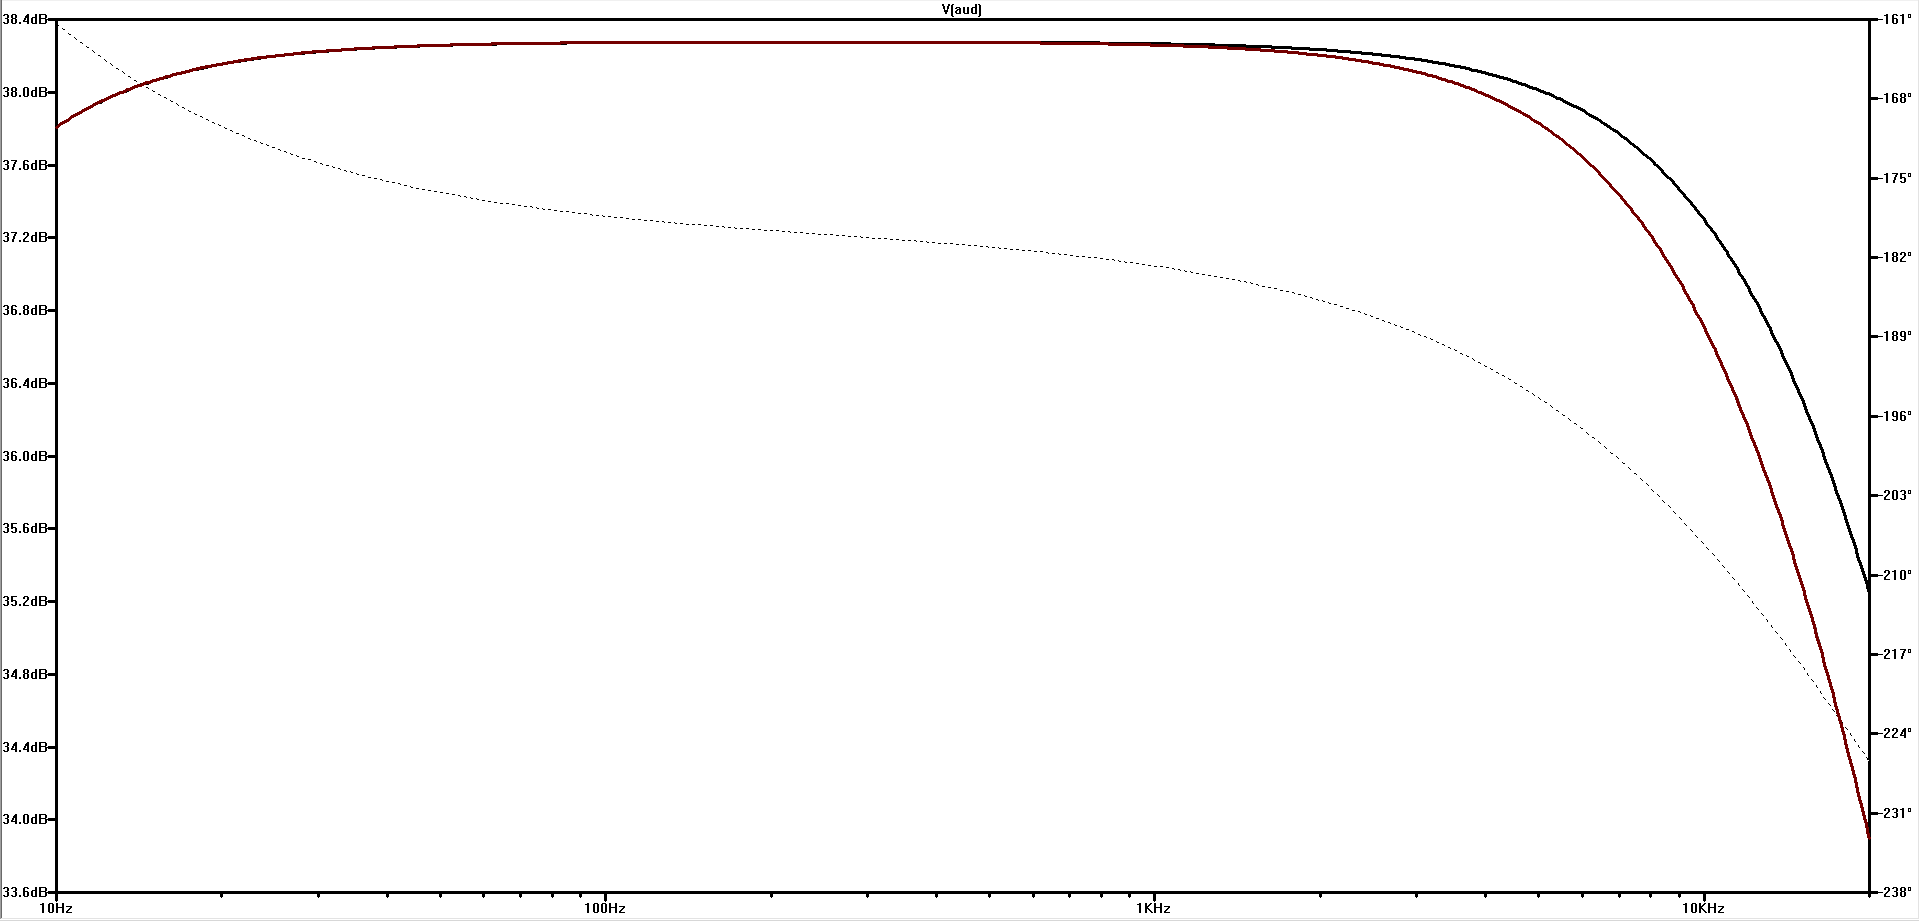
\includegraphics[width=0.75\textwidth]{figs/freq.png}}
\end{center}
\caption{\label{fig:freq} Frequency response of the microphone IC.}
\end{figure}

Suppose we need to determine the frequency spectrum of sound, for example, in order to build a guitar tuner.  Conceptually, the guitar provides $f(t)$ and we simply wish to calculate the Fourier transform $\widetilde{f}(\omega)$.  The start time is arbitrary, so the phase information contained in the Fourier transform is meaningless, and so in fact we need only $|\widetilde{f}(\omega)|^2$.

But our electronics cannot provide a continuous function $f(t)$.  Instead, we can only sample the microphone at discrete intervals separated by the sampling period $\tau$.  We have limited time and buffer space, so we will only sample during a limited period $T$.  Instead of the Fourier Transform, we will be calculating the discrete Fourier series.

Our time series data will consist of $n$ microphone values $x_j$, collected during a time interval of duration $T = n\tau$, and approximately evenly spaced.    Let's start with the Fourier Series for a function of time with period $T$.  In this case, neglecting the overall normalization, which we don't care about, the formula for calculating the Fourier coefficients is:
\begin{eqnarray*}
A_m &=&  \int_{-\frac{T}{2}}^{\frac{T}{2}} 
f(x) \cos\left(\frac{2\pi m}{T} \, t \right) \, dt \\
B_m &=& \int_{-\frac{T}{2}}^{\frac{T}{2}} 
f(x) \sin\left(\frac{2\pi m}{T} \, t \right) \, dt
\end{eqnarray*}
we can describe our discrete data sample, however, as:
\begin{equation*}
f(t) \to \sum_{i=0}^n \delta(t-i\tau) x_i
\end{equation*}
that is, it is zero everywhere but at the $n$ sample points, each at location $i\tau$ in time, where the value is $x_i$.
The delta function replaces the integrals above with sums, and the coefficients are now given by:
\begin{eqnarray*}
A_m &=&  \sum_{i=0}^n x_i  \cos\left(\frac{2\pi m}{n} \, i \right) \\
B_m &=&  \sum_{i=0}^n x_i  \sin\left(\frac{2\pi m}{n} \, i \right) \\
\end{eqnarray*}
Recall that the frequency associated with each $m$ is $f_m = m / T$.  Therefore, our lowest frequency (for $m=1$) is $f=1/T$.  From the Nyquist theorem, the highest frequency we can reliably sample is one half the sampling rate ($1/nT$) and therefore we'll have Fourier series coefficients for the frequencies:
\begin{displaymath}
f_m = \frac{m}{T} \; \; \; {\rm for} \; m=1,2,3,\ldots,\frac{n}{2}
\end{displaymath}
There are more computationally efficient ways to calculate the Discreet Fourier Series which are known collectively as a Fast Fourier Transform.   But we won't need to understand these algorithms as they merely reproduce the conceptually simple computation above (though much much faster).  We'll be using the periodogram feature of Scientific Python, which reports $\sqrt{A_m^2 + B_m^2}$ for each $f_m$, that is, with the arbitrary phase information removed.

Now let's look at particulars of our specific case.  With the Arduino in free running mode, the ADC sample rate is $76.9~\rm kHz$ which puts the Nyquist frequency at $33~\rm kHz$.  Any signal above this frequency would lead to aliasing.  Fortunately, this is well above the audio range and the microphone acts as a low-pass filter (see Fig.~\ref{fig:freq}), eliminating any risk of aliasing from higher frequency signals.

There's enough room in the Arduino for a 1500 byte buffer.  Therefore, our period for signal collection is 
{19.5~\rm ms}.  Our lowest frequency (for $m=1$) is $51.26~\rm Hz$ and our next lowest (for $m=2$) is $102.5~\rm Hz$.   That is actually pretty poor resolution for tuning a guitar, but we'll live with it for now.  A way around this limitation using a digital low pass filter is discussed in the Improvements section.

\section{Hardware Overview}

\begin{figure}[htbp]
\begin{center}
{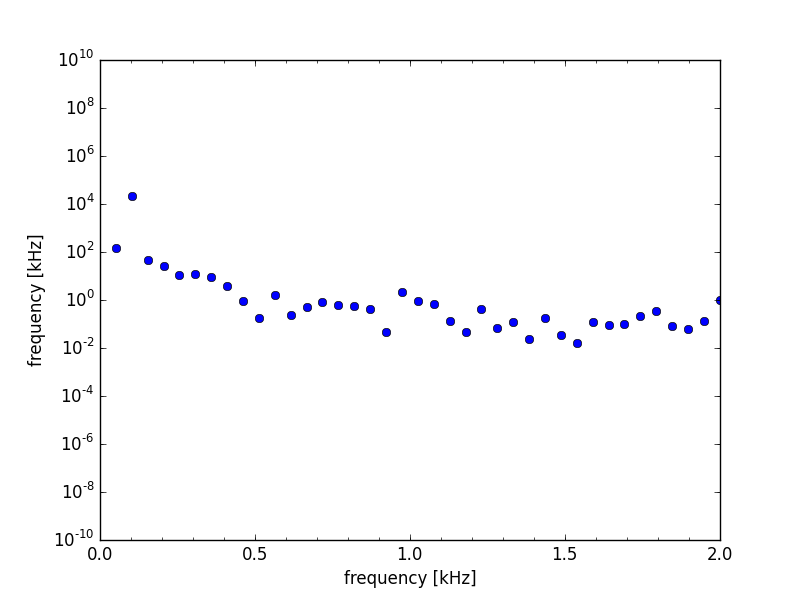
\includegraphics[width=0.55\textwidth]{figs/poor100hz.png}} \\
{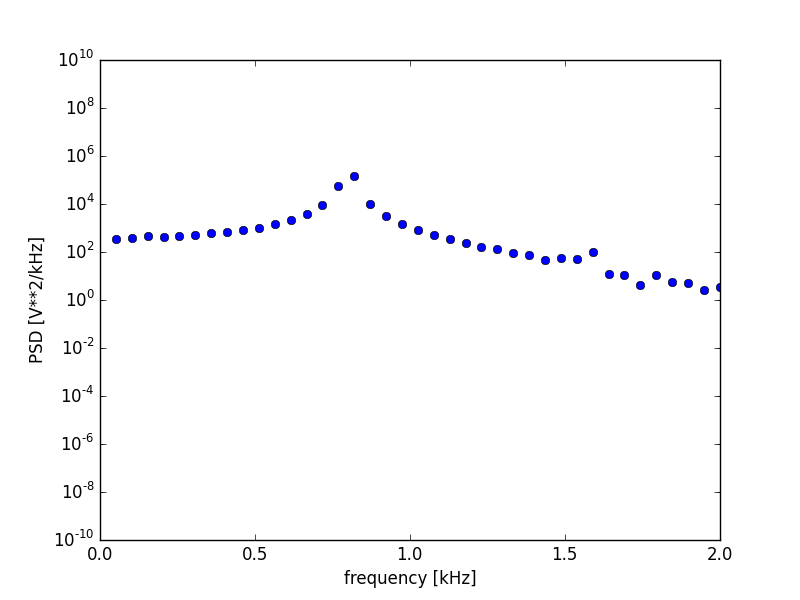
\includegraphics[width=0.55\textwidth]{figs/poor800hz.png}}\\
{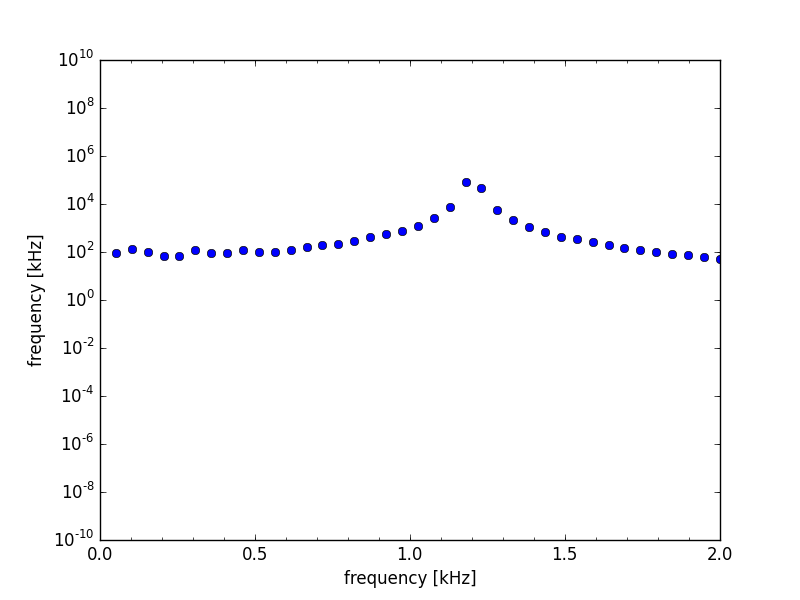
\includegraphics[width=0.55\textwidth]{figs/poor1200hz.png}}
\end{center}
\caption{\label{fig:firstpass} The spectrum analyzer tested with 100, 800 and 1200 Hz tones.  (The resolution and noise can both be further improved, as discussed in the Improvements section.)}
\end{figure}

In this lab, you will learn about hardware integration.  Most interesting technical feats are broken down into manageable components, often designed by different teams.  Someday, you may have the challenging job of integrating your colleagues components together into a working system.   The systems that your colleagues (aka me) will provide are:
\begin{itemize}
\item A microphone IC, with $5~\rm V$ output, specifically designed for use with the Arduino.
\item An Arduino Digital Scope sketch (Scope), which demonstrates how to sample the microphone.
\item An Arduino serial data service sketch (SerialDataService) which, upon request over the serial interface, fills a buffer with fake data and reports it on the serial interface.
\item A scientific python driver (serial\_driver.py), which requests data from the serial data service and plots it.
\item A Scientific Python code snippet demonstrating the scientific python Periodogram feature, which reports the magnitude of the Fourier coefficients for a discreetly sampled waveform.
\end{itemize}

Your job will be to put all of these working components\footnote{Here we differ from the real world, where often you get components that don't work as intended!} together and construct an audio spectrum analyzer. 
But first, you should work your way through the individual independent modules, and check that you can get them to work properly.  Then, when each individual module is working, you can begin the task of integrating the entire system.

\section{Microphone IC}

The microphone IC (Fig.~\ref{fig:mic}) includes a microphone and a gain 60 pre-amplifier.  This IC is designed for use with Arduino.  You simply connect VCC to a $5~\rm V$ pin, GND to a ground pin.  AUD is audio output in the $0$ to $5~\rm V$ range, suitable for sampling with an analog input (we will use A0).

To test your microphone initially, connect VCC and GND to the appropriate pins on the Arduino, but measure AUD  directly with your scope, as in Fig.~\ref{fig:micard}.  (The scope grounding clip should be connected to the Arduino ground while making this measurement.)  Whistling should produce a decent sine wave, as in Fig.~\ref{fig:whistlescope}.  If you can't whistle, you can find a fixed tone generator online.

\begin{figure}[htbp]
\begin{center}
{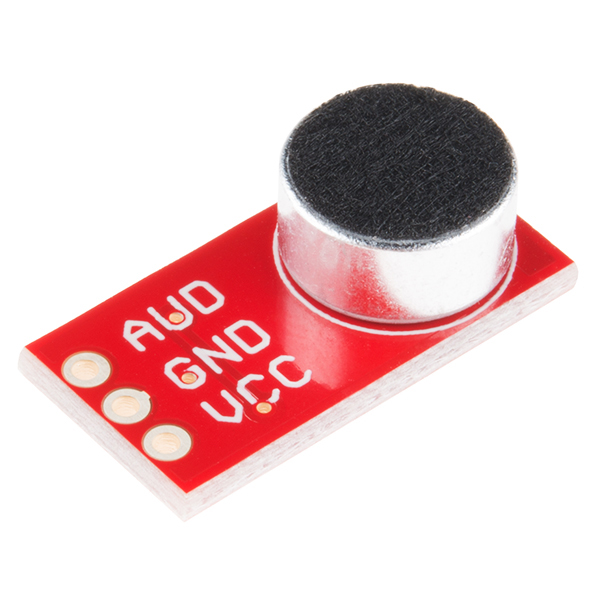
\includegraphics[width=0.20\textwidth]{figs/mic.jpg}}
\end{center}
\caption{\label{fig:mic} The microphone, with preamplifier (not shown) on the underside of the IC.}
\end{figure}

\begin{figure}[htbp]
\begin{center}
{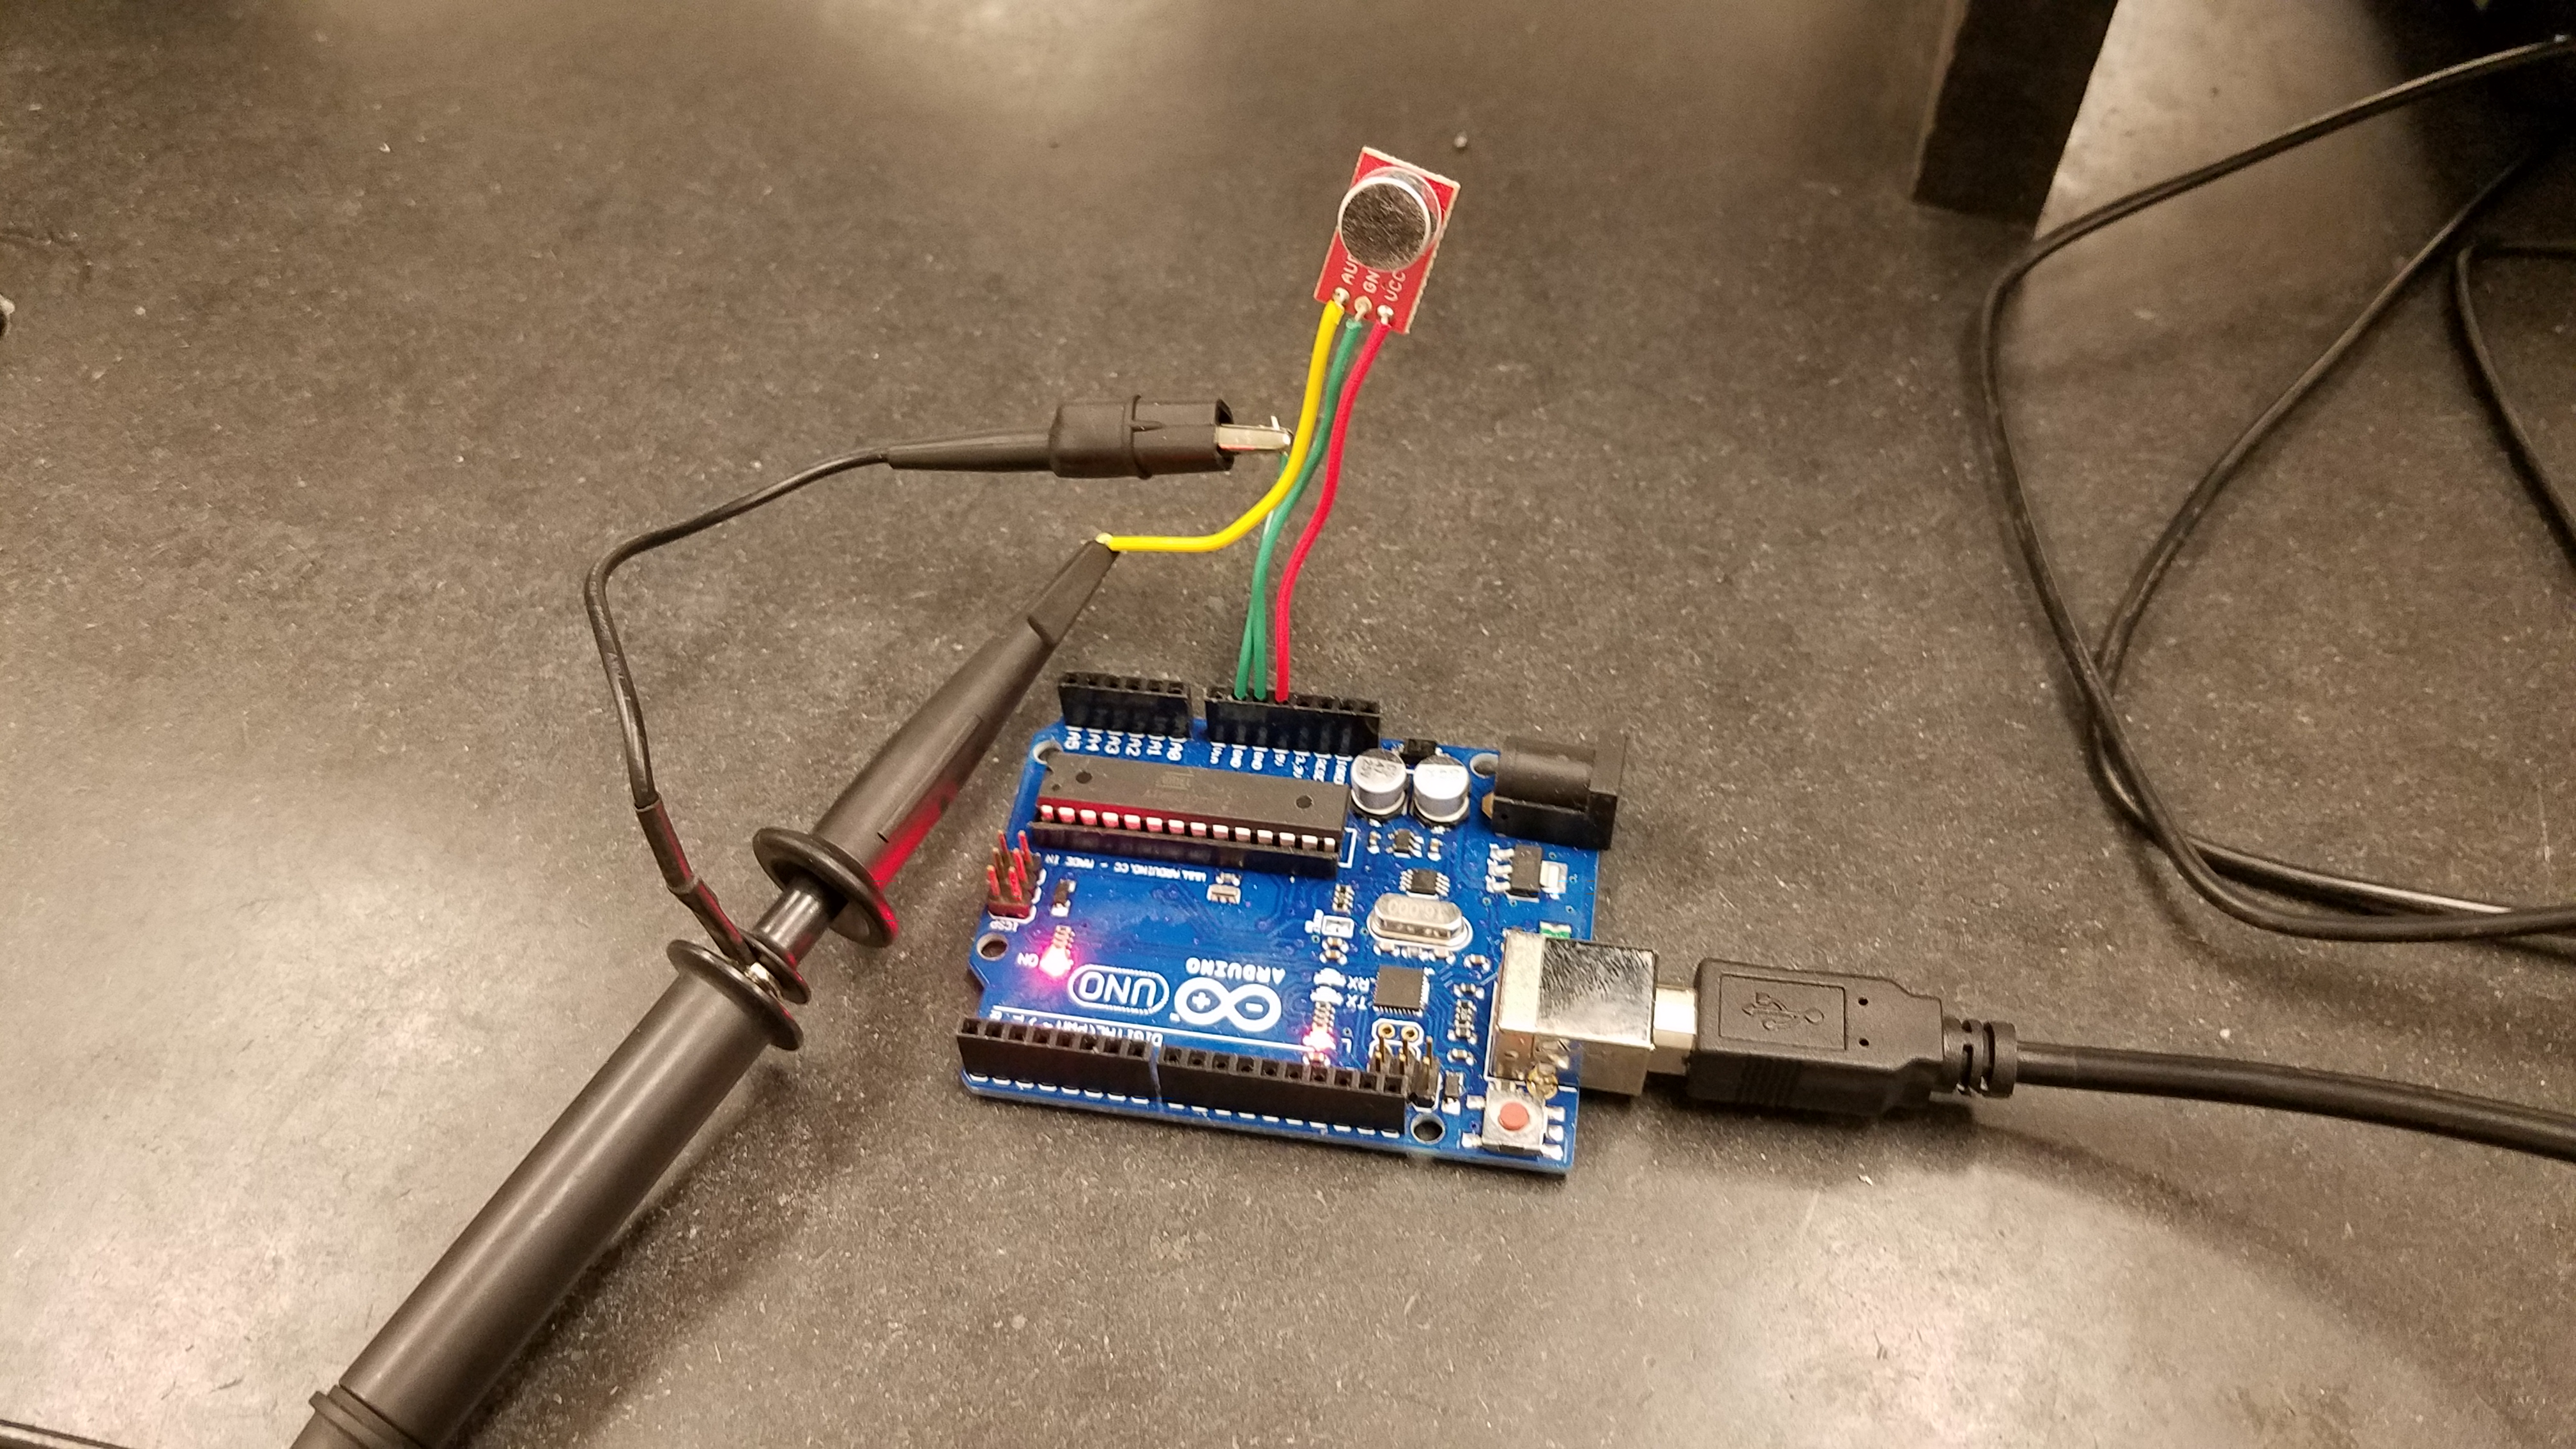
\includegraphics[width=0.70\textwidth]{figs/mic_ard.jpg}}
\end{center}
\caption{\label{fig:micard} The microphone powered by Arduino connected to oscilloscope probe.}
\end{figure}

\begin{figure}[htbp]
\begin{center}
{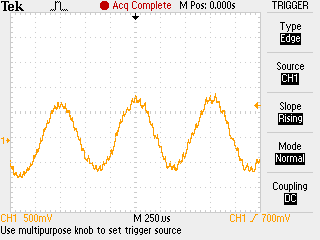
\includegraphics[width=0.70\textwidth]{figs/whistle_scope.png}}
\end{center}
\caption{\label{fig:whistlescope} Microphone audio output as observed on oscilloscope while whistling.}
\end{figure}

\section{Scope Sketch}

The scope sketch is much like it was for the Arduino Digital Sketch lab.  There's a section for configuring the ADC for free-running mode using low-level Arduino hardware driver code, located inside the setup: 
\begin{verbatim}
 ADCSRA = 0;             // clear ADCSRA register
 ADCSRB = 0;             // clear ADCSRB register
 ADMUX |= (adc & 0x07);    // set A(adc) analog input pin
 ADMUX |= (1 << REFS0);  // set reference voltage
 ADMUX |= (1 << ADLAR);  // left align ADC value to 8 bits from ADCH register
 // sampling rate is [ADC clock] / [prescaler] / [conversion clock cycles]
 // for Arduino Uno ADC clock is 16 MHz and a conversion takes 13 clock cycles
 ADCSRA |= (1 << ADPS2);                     // 16 prescaler for 76.9 KHz
 ADCSRA |= (1 << ADATE); // enable auto trigger
 ADCSRA |= (1 << ADIE);  // enable interrupts when measurement complete
 ADCSRA |= (1 << ADEN);  // enable ADC
 ADCSRA |= (1 << ADSC);  // start ADC measurements
\end{verbatim}
The {\tt adc} variable specifies which analog input to digitize.  It is set to 0 in the sketch, indicated Analog input 0 (A0).

There is also the all-important interrupt service routine, for processing the samples:
\begin{verbatim}
ISR(ADC_vect){
  if (isamp < max_samples){
    buf[isamp]=ADCH;
    isamp++;      
  }
}    
\end{verbatim}
In ADC free-running mode, this interrupt is called every time the hardware indicates that a new ADC value is available.  As implemented here, the interrupt simply stores the ADC value in the array {\tt buf} used to buffer the data, incrementing the index within the buffer, until the buffer is full.  For this lab, there is no need to implement a trigger, as we do not care about the phase of the waveform.

The Scope sketch does not implement the serial port interface we will be using to drive the data acquisition from the PC, as that feature was designed by another colleague.  Instead, whenever the buffer is full, it sends the first 500 samples to the serial port, suitable for easy plotting using the built-in serial plotter tool.  

Connect the microphone IC audio input to the appropriate Arduino input pin, load the Scope sketch, and start the serial plotter tool.   Whistle and confirm that you observe a sine wave, as in Fig.~\ref{fig:whistle}.
At this point you've integrated the microphone IC and the Arduino.

\begin{figure}[htbp]
\begin{center}
{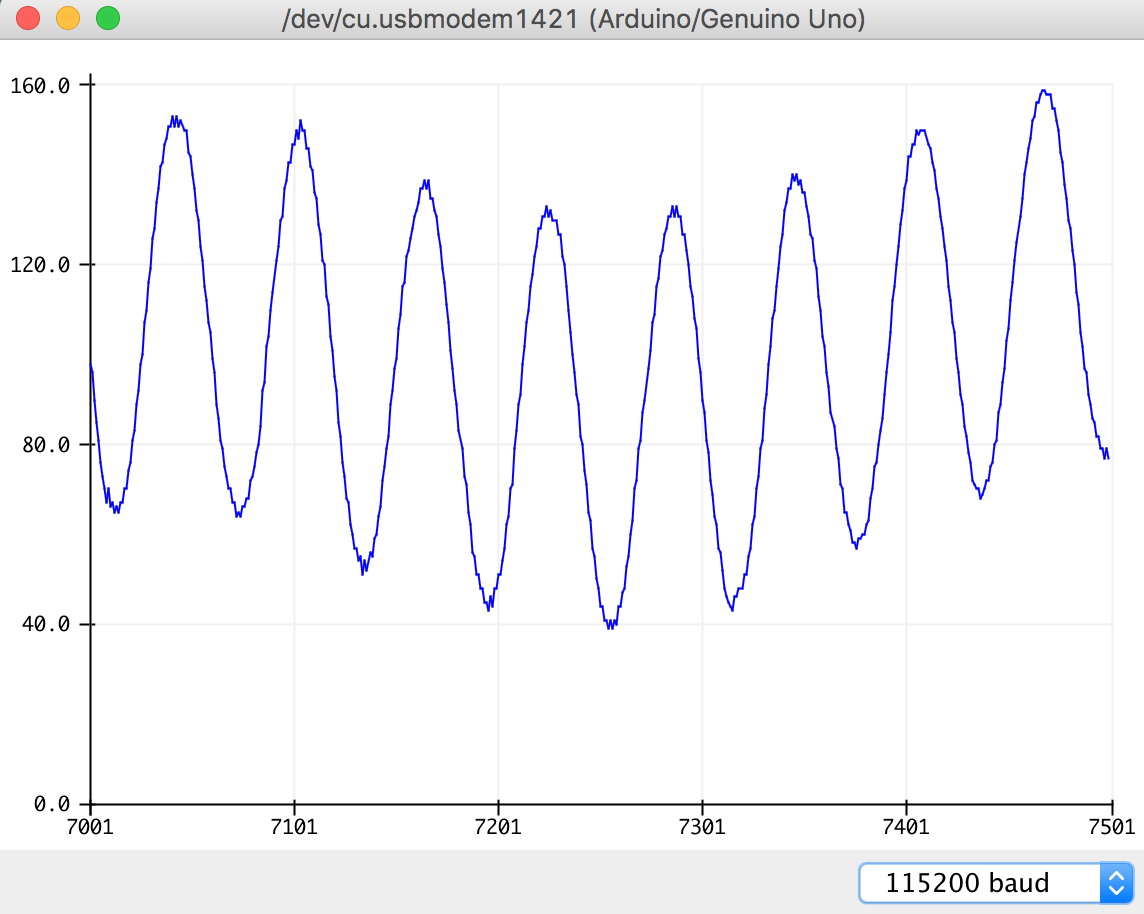
\includegraphics[width=0.75\textwidth]{figs/whistle.png}}
\end{center}
\caption{\label{fig:whistle} A whistle as observed on Serial Monitor using the Scope sketch.}
\end{figure}

\section{Serial Data Service Sketch}


The Serial Data Service sketch implements the Arduino side of the PC$\leftrightarrow$Arduino serial interface which will allow us to drive the DAQ on the Arduino from the PC.  

The Arduino sends a message to the serial link after its initialization is complete.  It then waits until it receives an acquire command over the serial interface (char 'a' over the serial link).  

 Upon receiving the acquire signal, the data buffer buf[] is reset to empty by setting the buffer index isamp to zero and the acquire flag is set to true.  Because your colleague who wrote this piece was not responsible for filling the buffer with actual measured data from the ADC, this sketch fills the buffer with test pattern data calculated from the sine function.  

 When the buffer is full and the acquire signal is true, the collected data is output over the serial port.
 The number of samples (max\_sample) collected is sent (initially set to 10, but can be changed).  Then the 
  data is sent, one measurement per line, with each line containing an index (0 to max\_sample) and the buffer value
  at that index.  You can think of this as t and f(t) at max\_sample discrete locations.
  After sending the entire data, the acquire flag is set to false, indicating that the request has been handled, and the Arduino will simply wait for the next request.

The driver interface uses the special function {\tt serialEvent()}.  This function is called after the loop function exits only if new serial data is available at the input:
\begin{verbatim}
void serialEvent() { 
  delay(1000);
  char inChar = (char) Serial.read();
  if (inChar == 'a'){
      isamp = 0;
      acquire = true;
  }
}
\end{verbatim}
The acquire command is indicated from the single character ``a", which sets the buffer to empty to cause fresh data to be sampled (in this case, a test pattern).  The acquire flag is set to true, indicating that data has been requested and should be sent to the serial port when the buffer is full.  This functionality is handled in the loop: 
\begin{verbatim}
void loop() {    
  // fill buffer with test pattern data if it is empty:
  fill_buffer_with_test_pattern();

  // if an acquire signal has been received, and the buffer is full, write the contents:
  if (acquire & (isamp == max_samples)) {
    write_buffer_to_serial_port();
    acquire = false;
  }
}
\end{verbatim}
The output to the serial interface starts with a simple ``header" specifying the number of samples in each waveform {\tt max\_samples} followed by a line for each sample indicating the index of the sample and the ADC value (an integer from 0 to 255 encoding 0 to $5~\rm V$):  
\begin{verbatim}
// write the contents of a full buffer on the serial port:
void write_buffer_to_serial_port(){
    // write header only for the first sample:
    Serial.println(max_samples);
    // write payload:
    for(int i=0; i<max_samples; i++){
      char line[100];
      sprintf(line, "%d %d", i, buf[i]);
      Serial.println(line);
      Serial.flush();
    }
}
\end{verbatim}

Test out the serial driver interface by hand in the serial monitor by sending the ascii command ``a' as in Fig.~\ref{fig:send}.  The reply from the Arduino is in  Fig.~\ref{fig:reply}.
\begin{figure}[ht bp]
\begin{center}
{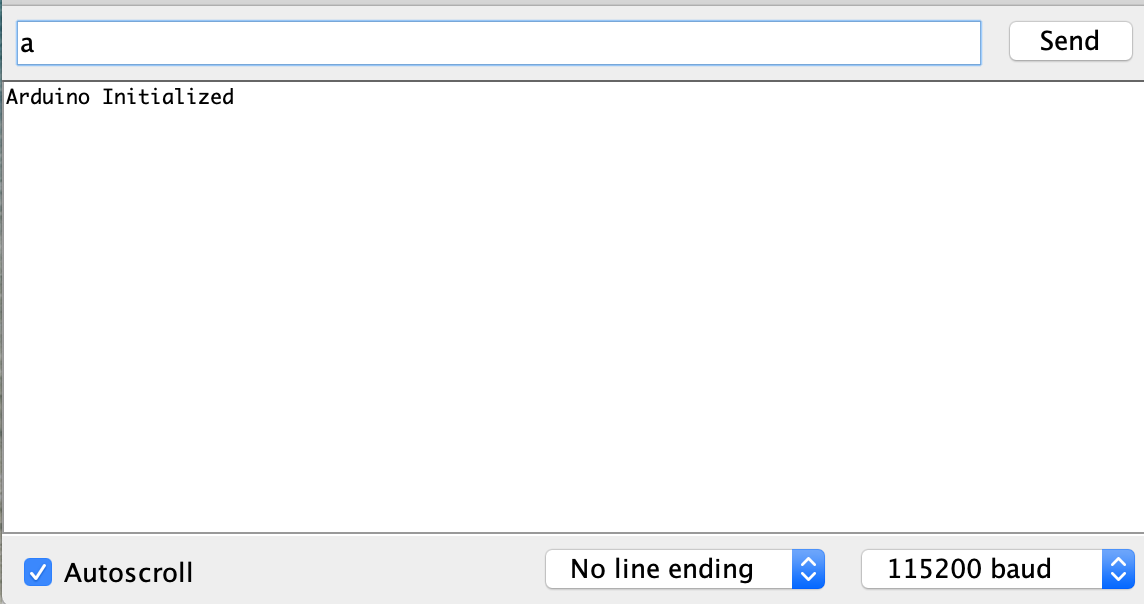
\includegraphics[width=0.75\textwidth]{figs/send.png}}
\end{center}
\caption{\label{fig:send} Sending the acquire command .}
\end{figure}
\begin{figure}[htbp]
\begin{center}
{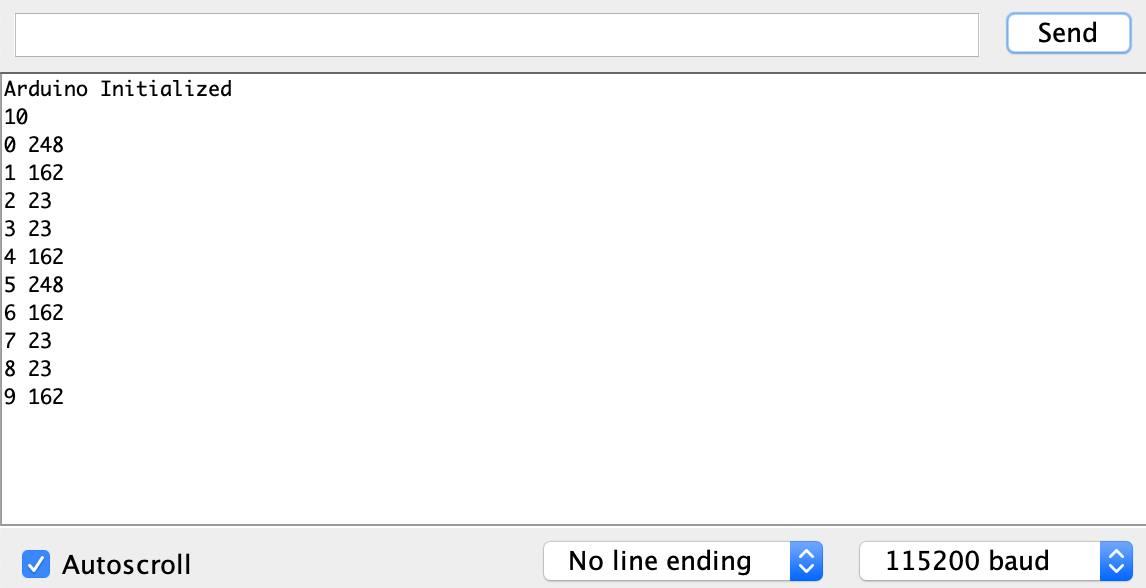
\includegraphics[width=0.75\textwidth]{figs/reply.png}}
\end{center}
\caption{\label{fig:reply} The Arduino reply.}
\end{figure}
The buffer size ({\tt max\_samples} is set to ten initially, to avoid overwhelming you with output when testing in the serial monitor.  Once you have tested this, you can increase the buffer size by setting {\tt max\_samples} to 1500. 

\section{Python Serial Driver Code}
The python serial driver code {\tt serial\_driver.py} is intended to be run on your PC.  From the Anaconda prompt in the directory where you have saved the {\tt serial\_driver.py} file, run the command:
\begin{verbatim}
ipython serial_driver.py
\end{verbatim}
The driver will first prompt you for the serial port that the Arduino is connected to.  If you get tired of being prompted for this, you can replace the prompt with a hard coded value, as in the commented lines above it:
\begin{verbatim}
#SERIAL_PORT="COM4"
#SERIAL_PORT="/dev/cu.usbmodem1421"
SERIAL_PORT=input("Enter the serial port for the Arduino (e.g. COM4):  ")
\end{verbatim}
If you encounter permission errors while accessing the COM port, it is likely that you have left a serial monitor open, which claims exclusive ownership.

The important part of the serial driver python code is the interaction with the Arduino over the serial port:
\begin{verbatim}
ser.write(str.encode("a"))
# first line is the length of the payload:
nsamp = int(ser.readline().strip().decode("ASCII"))

t_dat = np.zeros(nsamp, dtype=float)
f_dat = np.zeros(nsamp, dtype=float)
print("receiving payload from Arduion of length ", nsamp, "\n")

for i in range(nsamp):
        str = ser.readline().strip().decode("ASCII")
        t,f = str.split()
        if (i<5):
                print("t: ", t, "f(t): ", f)
        t_dat[i] = float(t)
        f_dat[i] = float(f)
ser.close()
\end{verbatim}
Here it sends the acquire command, then reads the Arduino reply, which starts with the number of samples.  The sample indices are stored in {\tt t\_dat} numpy array, which you can interpret as time stamps in units of $1/f_s$ where $f_s$ is the sample frequency of the Arduino ADC.  The ADC values, integers from 0 to 255 encoding 0 to 5~V, are stored in the {\tt f\_dat} array.  Because we only care about absolute frequency, we don't need to convert these to voltages.
  
\begin{figure}[htbp]
\begin{center}
{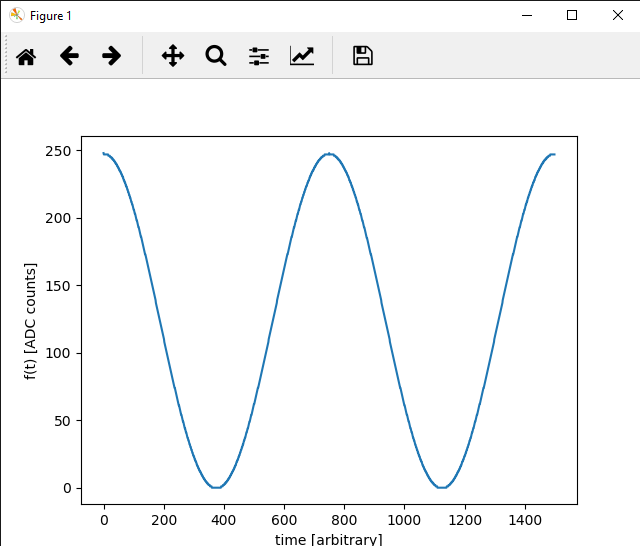
\includegraphics[width=0.75\textwidth]{figs/testpattern.png}}
\end{center}
\caption{\label{fig:wave} Test pattern from Arduino plotted in Scientific Python.}
\end{figure}


\section{Periodogram}

An example ipython notebook using scientific python to create a periodogram is also available on the course website.  First, a test pattern (sine wave) is filled, then the periodogram is calculated and plotted as in Fig.~\ref{fig:periodogram}.


\begin{figure}[htbp]
\begin{center}
{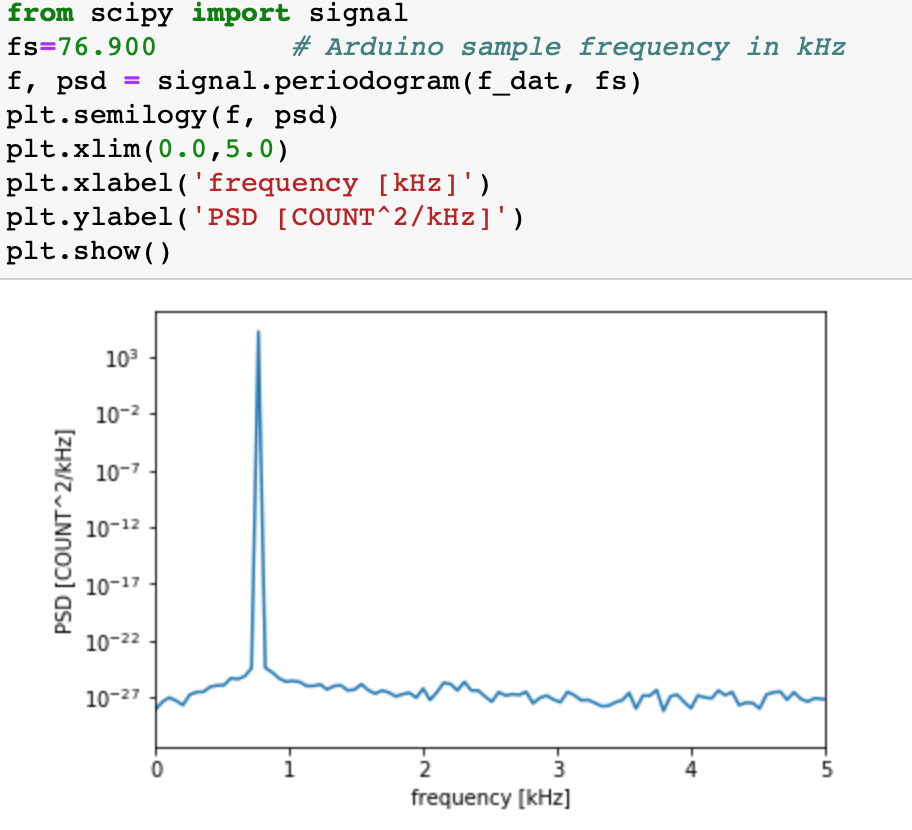
\includegraphics[width=0.65\textwidth]{figs/periodogram.png}}
\end{center}
\caption{\label{fig:periodogram} Periodogram from test pattern.}
\end{figure}

\section{Interfaces}

When dividing a system into several blocks, it's important for good design to think in terms of the interfaces between different functional blocks.  You want to design the block diagram for a system so that the interfaces are as simple as possible.  In this example, we have several interfaces between successive stages:
\begin{itemize}
\item The microphone IC and the Arduino have a hardware interface: VCC is connected to $5~\rm V$, GND to ground, and AUD to analog input 0 (A0).
\item The Scope and Serial Data Service share an interface through the data buffer implemented in C as the byte array {\tt byte buf[max\_samples]}.  The global variable {\tt isamp} points to the current location in data buffer.  When {\tt isamp} is zero, the buffer is empty, and when {\tt isamp} is equal to {\tt max\_samples}  the buffer is full and ready for readout.
\item The Arduino and the PC are connected by the serial interface, according to the simple protocol described above, wherein the PC requests a sample and the Arduino collects and transmits data back to the PC.
\item The PC serial driver code {\tt serial\_driver.py} and the periodogram analysis {\tt periodogram.ipynb} share an interface through the ADC sample data stored in the numpy array {\tt f\_dat}. 
\end{itemize}
By understanding the interfaces, you will know exactly how to connect each stage to the next.

\section{Integration}

Now you are ready to integrate the entire system.  By now you should have worked through the preceding sections so that you know each piece is working.  You should already have connected the microphone to the Arduino and seen that it is working with the Scope sketch.  You should also have tested the serial interface between the Arduino and the PC using the Serial Data Service sketch on the Arduino and the {\tt serial\_driver.py} code on the PC. 

There are only two main gaps in the whole chain: providing real data collected from the microphone to the serial interface, and adding the periodogram feature to the PC driver.  It's easiest to tackle the latter part first.  Make a copy of the {\tt serial\_data.py} file and call is something like {\tt psd\_driver.py} to contain your updates to the code.   Make a copy of the SerialDataService sketch and call it something like {\tt SerialScope}.  Without making any changes from the original code, first test that your new {\tt psd\_driver.py} code on the PC can receive the test pattern (a sine wave) from the Arduino running your new {\tt SerialScope} sketch.  In your {\tt SerialScope} make certain to set {\tt max\_samples} to 1500 on the Arduino for a nice smooth sine wave from many samples, as shown in Fig.~\ref{fig:wave}. 

 Next modify your {\tt psd\_driver.py} code to include the periodogram feature demonstrated in the {\tt periogram.ipynb} example, keeping in mind that their common interface is the {\tt f\_dat} array.  The periodogram for the low frequency sine wave in the test pattern should make a large peak at low frequency in the periodogram.
 
Once the periodogram feature is working, you are ready to tackle the last link.   You need to merge the appropriate code from the {\tt Scope} sketch, by cutting and pasting, into your {\tt SerialScope} sketch, which initially is simply a copy of {\tt SerialDataService}.  As described above, the interface between these two blocks is the data buffer implemented in C as the byte array {\tt byte buf[max\_samples]}.  The global variable {\tt isamp} points to the current location in data buffer.  When {\tt isamp} is zero, the buffer is empty, and when {\tt isamp} is equal to {\tt max\_samples}  the buffer is full and ready for readout.
You want to import, by cutting and pasting, the code from the {\tt Scope} sketch that {\bf writes} this buffer.  This is the ISR function and the setup related to ADC free-running mode.  You do not want to include anything from the {\tt Scope} sketch that accesses the serial port.  Now that you are retrieving real data from the ADC, you'll want to turn off (by commenting out) the call to {\tt fill\_buffer\_with\_test\_pattern()}.
With these changes, your {\tt SerialScope} sketch should provide digitized samples collected from the microphone to the PC, which will further analyze the data to produce the periodogram.

Example output from a working spectrum analyzer is shown in Fig.~\ref{fig:firstpass}.


\section{Further Improvements}

There are two improvements that you can pursue if you have time and interest.\\

\noindent
{\bf Frequency Resolution:}  We worked hard to get the ADC sampling rate as high as possible.  But, we are limited to about 1500 samples, and this limits our sampling period to about $19.5~\rm ms$ and our frequency resolution ($f_1$) to about $50~\rm Hz$.  That's enough to tell the difference between guitar strings, but not to tune them.

One way around this would be to simply lower the sampling rate.  As long as we keep the Nyquist rate above $10~\rm kHz$ (where the microphone cuts out) we don't have to worry about aliasing.  So we could simply skip two out of every three samples, increasing our frequency resolution to $16~\rm Hz$.

But there's something better we can do.  If we simply average $n$ samples and save that to the buffer, we produce, effectively a low-pass filter with a very sharp cutoff.  We are still sampling at the higher rate, so the Nyquist frequency remains comfortable high at around $30~\rm kHz$.  Averaging samples kills any frequency component between $30~\rm kHz$ and the Nyquist frequency for the reduced sampling rate.\\

\noindent
{\bf Boosting Signal To Noise:}  Averaging the periodograms from several waveforms should increase the signal to noise ratio by eliminating random noise.  

\begin{figure}[htbp]
\begin{center}
{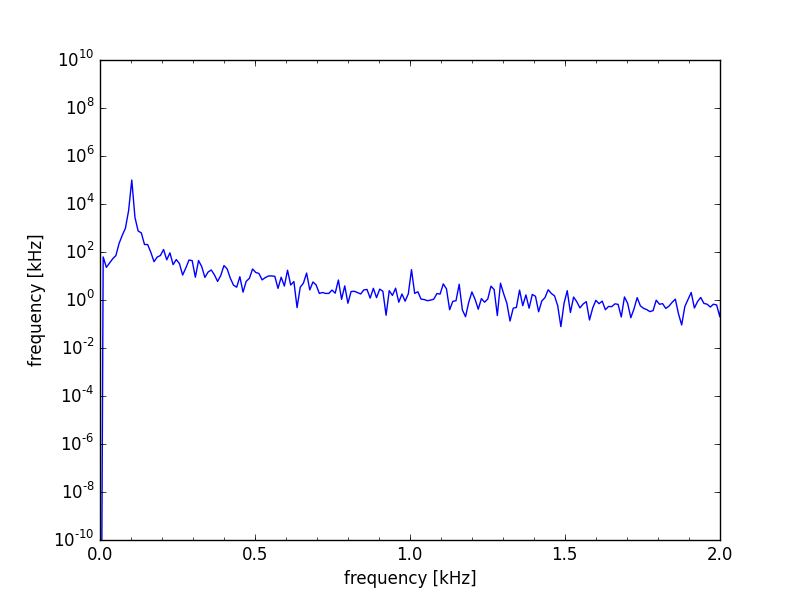
\includegraphics[width=0.65\textwidth]{figs/res100hz.png}} \\
{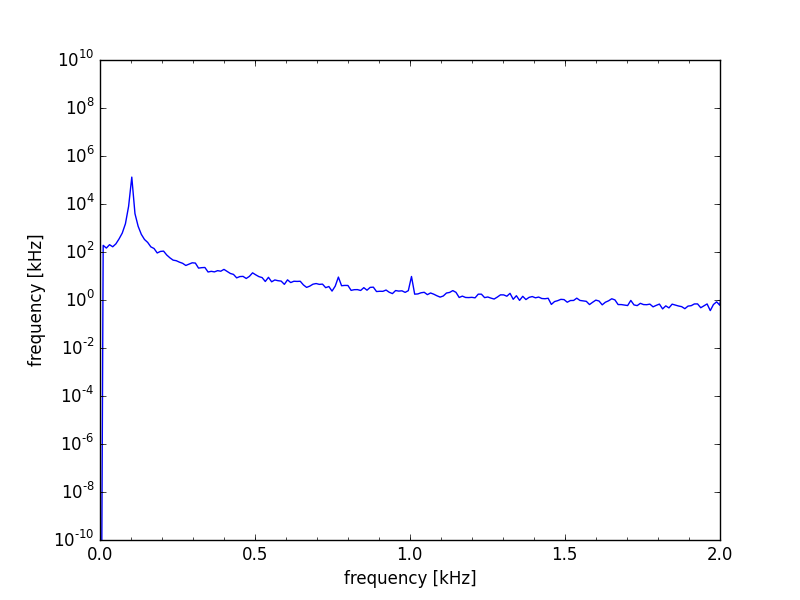
\includegraphics[width=0.65\textwidth]{figs/avg100hz.png}}
\end{center}
\caption{\label{fig:periodogram2} Periodogram for 100~Hz sound with (top) just resolution improvements, and (bottom) averaging to reduce background noise. }
\end{figure}



\end{document}


